\documentclass[12pt, a4paper]{article}

\usepackage[utf8]{inputenc}
% Limit the page margin to only 1 inch.
\usepackage[margin=1in]{geometry}

%Imports biblatex package
\usepackage[
backend=biber,
style=alphabetic
]{biblatex}
\addbibresource{../../algs4e.bib}

% Enables the `align' environment.
\usepackage{amsmath}
% Provides useful environments, such as:
% - \begin{proof} ...\end{proof}
\usepackage{amsthm}
\usepackage[most]{tcolorbox}

\newtheorem*{proposition}{Proposition}

% Enables using \mathbb{}, for example \mathbb{N} for the set of natural numbers.
\usepackage{amssymb}

% Allows using letters in enumerate list environment. Use, for example:
%\begin{enumerate}[label=(\alph*)]
% ...
%\end{enumerate}
\usepackage[inline]{enumitem}

% Enable importing external graphic files and provides useful commannds, like \graphicspath{}
\usepackage{graphicx}
% Images are located in a directory called images in the current directory.
\graphicspath{{./images/}}

% Make links look better by default.
% See: https://tex.stackexchange.com/questions/823/remove-ugly-borders-around-clickable-cross-references-and-hyperlinks
\usepackage[hidelinks]{hyperref}
\usepackage{xcolor}
\hypersetup{
	colorlinks,
	linkcolor={red!50!black},
	citecolor={blue!50!black},
	urlcolor={blue!80!black}
}


% Code Listings. Source:
% https://stackoverflow.com/questions/3175105/inserting-code-in-this-latex-document-with-indentation
\usepackage{listings}
\usepackage{color}

\definecolor{dkgreen}{rgb}{0,0.6,0}
\definecolor{gray}{rgb}{0.5,0.5,0.5}
\definecolor{mauve}{rgb}{0.58,0,0.82}

\lstset{frame=tb,
	language=Java,
	aboveskip=3mm,
	belowskip=3mm,
	showstringspaces=false,
	columns=flexible,
	basicstyle={\small\ttfamily},
	numbers=none,
	numberstyle=\tiny\color{gray},
	keywordstyle=\color{blue},
	commentstyle=\color{dkgreen},
	stringstyle=\color{mauve},
	breaklines=true,
	breakatwhitespace=true,
	tabsize=3
}

\newcommand{\prob}{\text{P}}
%\newcommand{\complement}{\mathsf{c}}

% Define an environment called "ex" (for Exercise) so that I can do: \begin{ex}{1.5}...\end{ex}
\newenvironment{ex}[2][Exercise]
{\par\medskip\noindent \textbf{#1 #2.}}
{\medskip}

% Define a solution environment, similar to ex (exercise) environment.
\newenvironment{sol}[1][Solution]
{\par\medskip\noindent \textbf{#1.} }
{\medskip}

\begin{document}
	\noindent Sergio E. Garcia Tapia \hfill
	
	\noindent \emph{Algorithms} by Sedgewick and Wayne (4th edition) \cite{sedgewick_wayne}\hfill
	
	\noindent December 31st, 2024\hfill 
	\section*{3.3: Balanced Search Trees}
	\begin{ex}{1}
		Draw the 2-3 tree that results when you insert the keys \texttt{E A S Y Q U T I O N}
		in that order into an initially empty tree.
	\end{ex}
	\begin{sol}
		See Figure~\ref{fig:ex-01}
		\begin{figure}
			\centering
			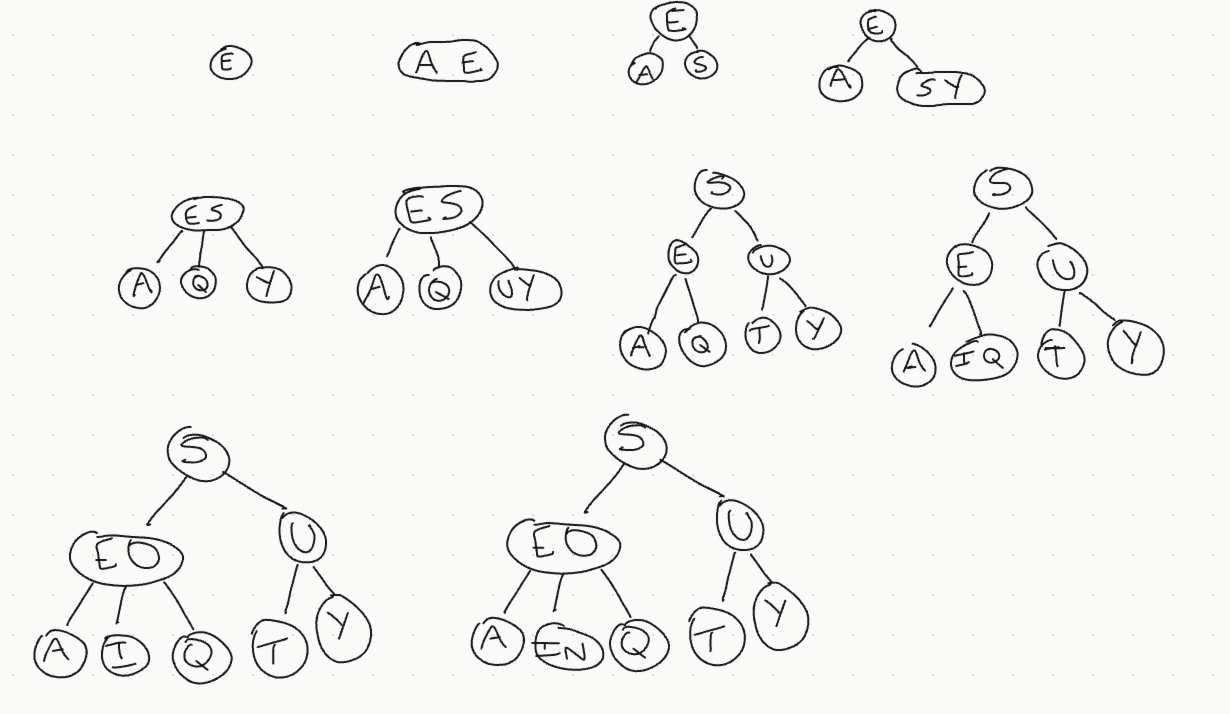
\includegraphics[width=0.7\textwidth]{exercise-01}
			\caption{Sequence of 2-3 trees when inserting the keys in Exercise 1.}
			\label{fig:ex-01}
		\end{figure}
	\end{sol}
	\begin{ex}{2}
		Draw the 2-3 tree that results when you insert the keys
		\texttt{Y L P M X H C R A E S} in that order into an initially empty tree.
	\end{ex}
	\begin{sol}
		See Figure~\ref{fig:ex-02}
		\begin{figure}
			\centering
			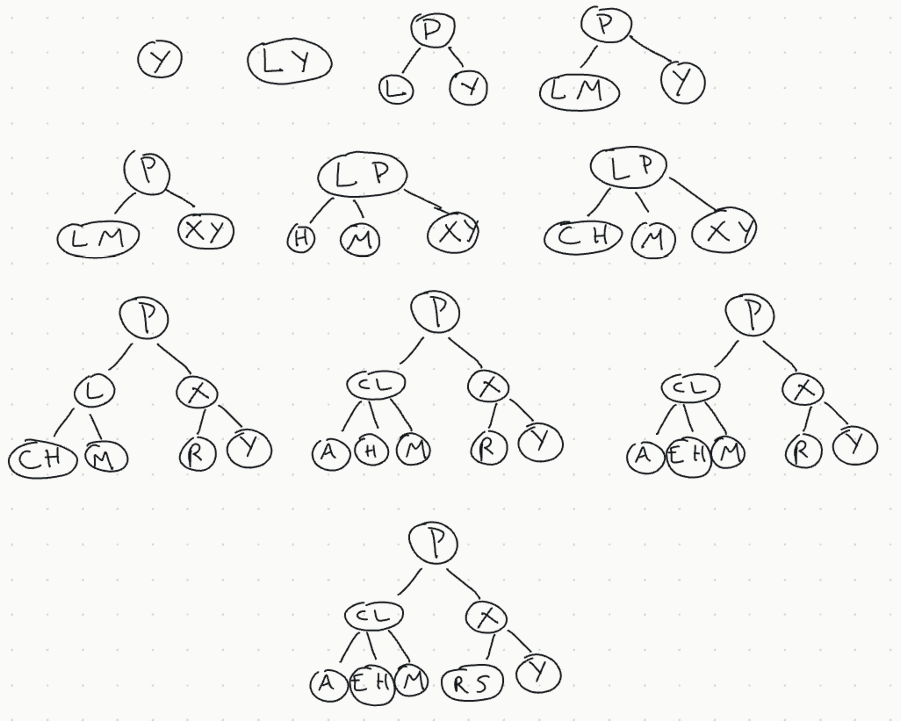
\includegraphics[width=0.6\textwidth]{exercise-02}
			\caption{Sequence of 2-3 trees when inserting the keys in Exercise 2.}
			\label{fig:ex-02}
		\end{figure}
	\end{sol}
	\begin{ex}{3}
		Find an insertion order for the keys \texttt{S E A R C H X M} that leads to a
		2-3 tree of height 1.
	\end{ex}
	\begin{sol}
		See Figure~\ref{fig:ex-03}.
		
		\begin{figure}
			\centering
			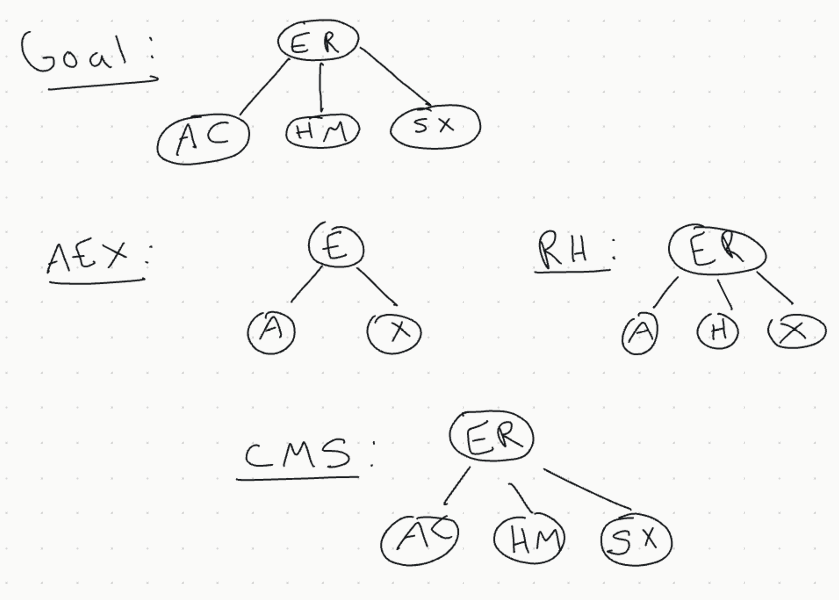
\includegraphics[width=0.6\textwidth]{exercise-03}
			\caption{Tree of height 1 for keys in Exercise 3.}
			\label{fig:ex-03}
		\end{figure}
		
		First, consider the the sort of the keys is \texttt{A C E H M R S X}.
		Since there are 8 keys, we can obtain a tree of height 1 if we have four 3-nodes.
		In particular, \texttt{E} and \texttt{R} are at the root, and \texttt{A} and \texttt{X}
		are in the leftmost and rightmost leaves, respectively. We can begin by inserting
		\texttt{AEX}, which places \texttt{E} at the root as desired. We can then insert
		\texttt{R} and \texttt{H}. Both fall in the rightmost leaf, and the split of the
		4-node that is created causes \texttt{R} to move to the root node, and the
		creation of the new leaf \texttt{H}. Now inserting \texttt{C} yields the 3-node
		with \texttt{A} and \texttt{C}, inserting \texttt{M} yields the node with \texttt{H} and
		\texttt{M}, and inserting \texttt{S} yields the node with \texttt{S} and \texttt{X}.
	\end{sol}
	\begin{ex}{4}
		Prove that the height of a 2-3 tree with $n$ keys is between $\lfloor \log_3n\rfloor
		\approx 0.63\lg n$ (for a tree that is all 3-nodes) and $\lfloor \lg_n\rfloor$
		(for a tree that is all $2$-nodes).
	\end{ex}
	\begin{sol}
		\begin{proof}
			Suppose $T$ is a 2-3 search tree. By construction, a 2-3 search tree is
			perfectly balanced, so $T$ is perfectly balanced also. In the worst case, if
			$T$ consists of only 2-nodes, then it will have $2^k$ nodes at all depths
			(except possibly the last one) because it is balanced. Similarly, in the best
			case, if $T$ consists only of 3-nodes then it will have $3^k$ nodes at all
			depths (except possibly the last one). The former tree has a height of
			$\lfloor \lg_n\rfloor$, and the latter has a height of $\lfloor \log_3 n\rfloor$.
			We conclude that $T$'s height lies in between the two.
		\end{proof}
	\end{sol}
	\begin{ex}{5}
		Figure~\ref{fig:ex-05-1} shows all the \emph{structurally different} 2-3 trees with $n$
		keys, for $n$ from 1 up to 6 (ignore the order of the subtrees). Draw all the structurally
		different trees for $n=$ $7$, $8$, $9$, and $10$.
		\begin{figure}
			\centering
			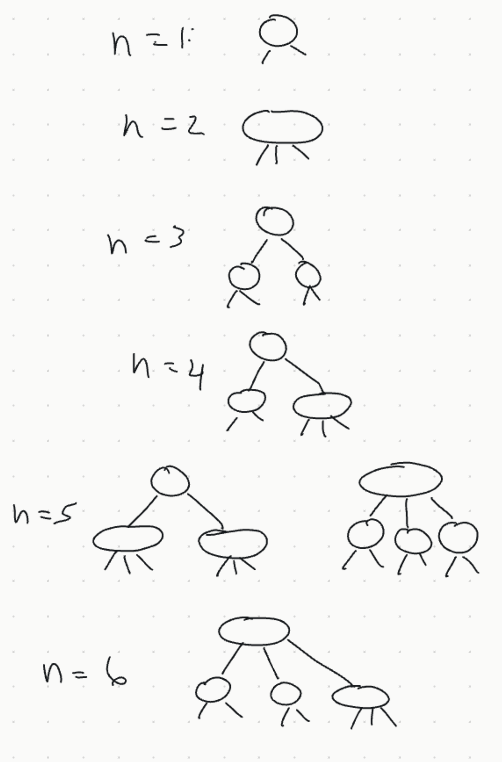
\includegraphics[width=0.4 \textwidth]{exercise-05-1}
			\caption{All of the structurally different 2-3 trees with $n$ keys, for
			$n$ from 1 through $6$.}
			\label{fig:ex-05-1}
		\end{figure}
	\end{ex}
	\begin{sol}
		See Figure~\ref{fig:ex-05-2}.
		\begin{figure}
			\centering
			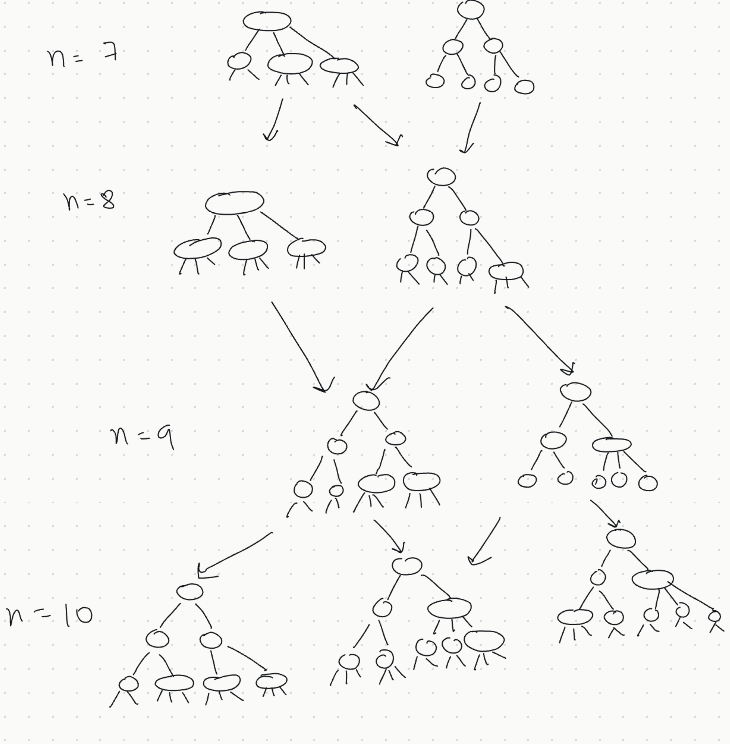
\includegraphics[width=0.6\textwidth]{exercise-05-2}
			\caption{All of the structurally different 2-3 trees with $n$ keys, for
				$n$ from $7$ through $10$.}
			\label{fig:ex-05-2}
		\end{figure}
	\end{sol}
	\begin{ex}{6}
		Find the probability that each of the 2-3 trees in Exercise 3.3.5 is the result
		of the insertion of $n$ random distinct keys into an initially empty tree.
	\end{ex}
	\begin{sol}
		See Figure~\ref{fig:ex-06-1} and Figure~\ref{fig:ex-06-2}, both of which I
		have annotated. Note that when a given tree can lead to more than one structurally
		different tree, I have annotated the arrows indicating the probability with
		which it can give rise to said structure. This ``transitional probability"
		then plays a role in the computation of the probabilities of the resulting tree.
		\begin{figure}
			\centering
			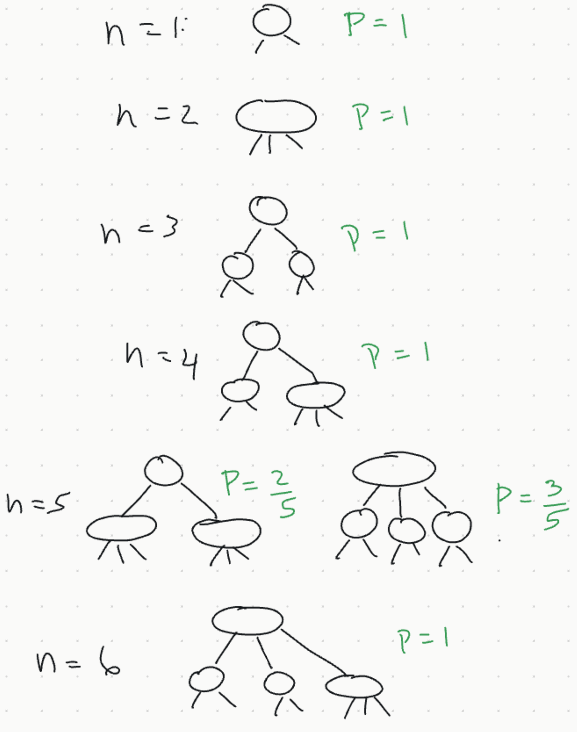
\includegraphics[width=0.6\textwidth]{exercise-06-1}
			\caption{All of the structurally different 2-3 trees with $n$ keys, for
				$n$ from $1$ through $6$ and their probabilities.}
			\label{fig:ex-06-1}
		\end{figure}
		\begin{figure}
			\centering
			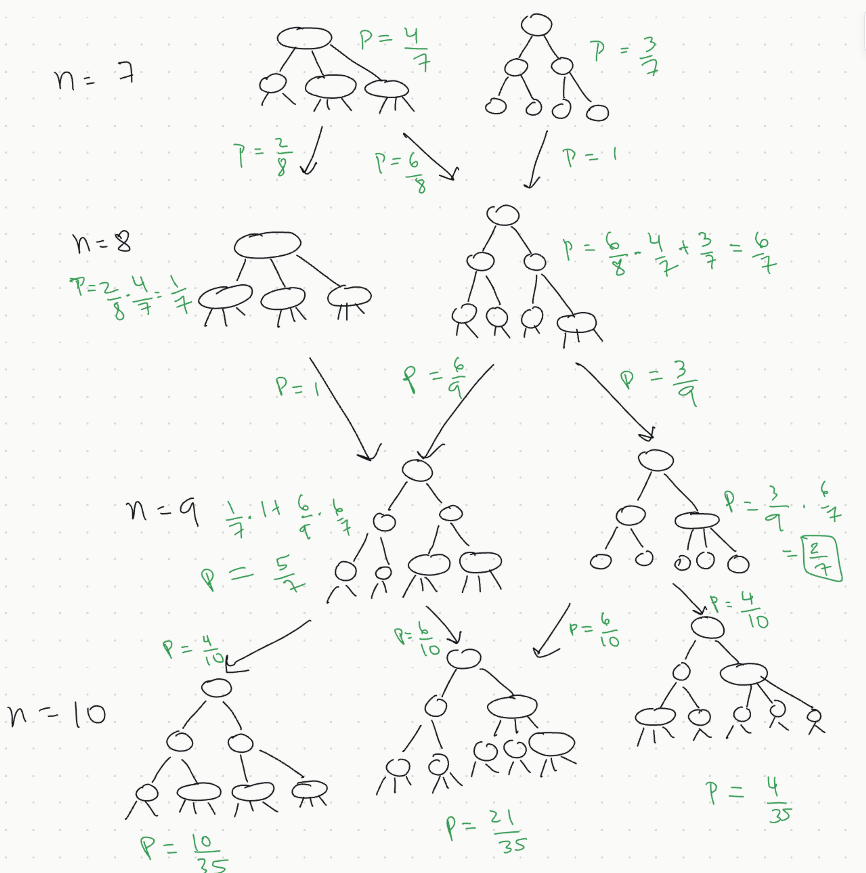
\includegraphics[width=0.7\textwidth]{exercise-06-2}
			\caption{All of the structurally different 2-3 trees with $n$ keys, for
				$n$ from $7$ through $10$ and their probabilities.}
			\label{fig:ex-06-2}
		\end{figure}
	\end{sol}
	\begin{ex}{8}
		Show all possible ways that one might represent a 4-node with three 2-nodes
		bound together with red links (not necessarily left-leaning).
	\end{ex}
	\begin{sol}
		See Figure~\ref{fig:ex-08}.
		\begin{figure}
			\centering
			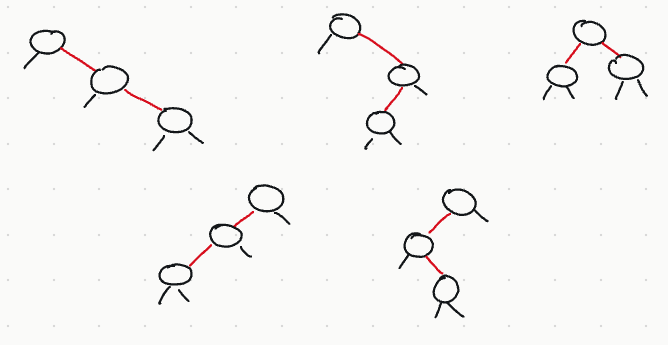
\includegraphics[width=0.6\textwidth]{exercise-08}
			\caption{All ways to represent a 4-node with three 2-nodes bound by red links.}
			\label{fig:ex-08}
		\end{figure}
	\end{sol}
	\begin{ex}{9}
		Which of the trees in Figure~\ref{fig:ex-09} are red-black BSTs?
		\begin{figure}
			\centering
			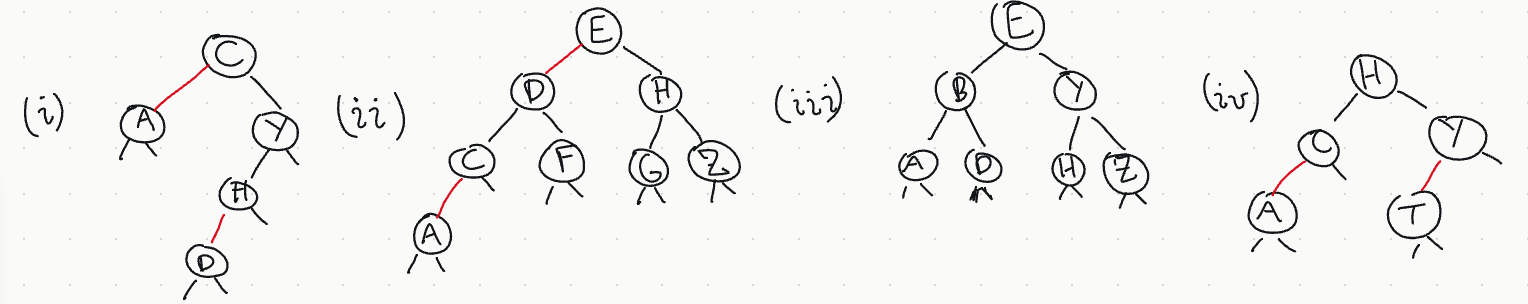
\includegraphics[width=0.9\textwidth]{exercise-09}
			\caption{Options for Exercise 9.}
			\label{fig:ex-09}
		\end{figure}
	\end{ex}
	\begin{sol}
		 Tree (i) is not a red-black BST because it does not have perfect black balance.
		 Tree (ii) is not a red-black BST because it is not ordered. In particular,
		 \texttt{F} is on the left subtree of \texttt{E} instead of right. The remaining
		 trees are red-black BSTs.
	\end{sol}
	\begin{ex}{10}
		Draw the red-black BST that results when you insert items with the keys
		\texttt{E A S Y Q U T I O N} in that order into an initially empty tree.
	\end{ex}
	\begin{sol}
		 See Figure~\ref{fig:ex-10}.
		 \begin{figure}
		 	\centering
		 	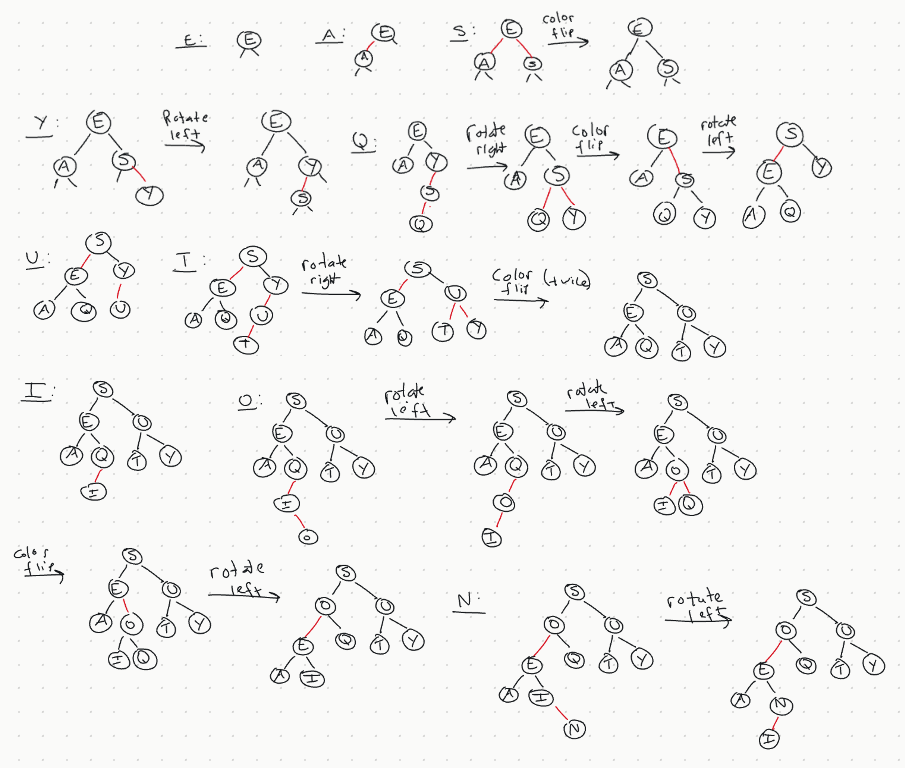
\includegraphics[width=0.9\textwidth]{exercise-10}
		 	\caption{Sequence of red-black BSTs generated by the key sequence in Exercise 10.}
		 	\label{fig:ex-10}
		 \end{figure}
	\end{sol}
	\begin{ex}{11}
		Draw the red-black BST that results when you insert the keys
		\texttt{Y L P M X H C R A E S} in that order into an initially empty tree.
	\end{ex}
	\begin{sol}
		By using the 1-1 corresponding of 2-3 trees and red-black BSTs, we can use the 2-3
		tree in Exercise 3.3.2 to create the corresponding red-black BST, depicted
		in Figure~\ref{fig:ex-11}.
		\begin{figure}
			\centering
			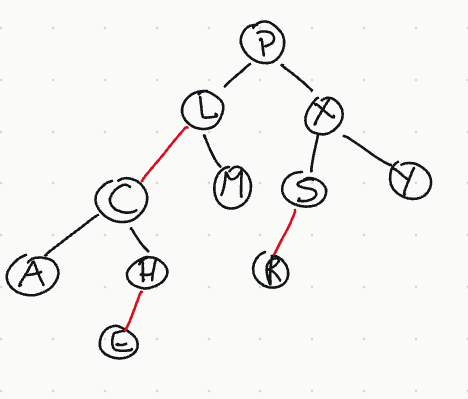
\includegraphics[width=0.4\textwidth]{exercise-11}
			\caption{Red-black BST resulting from the key sequence in Exercise 11.}
			\label{fig:ex-11}
		\end{figure}
	\end{sol}
	\begin{ex}{13}
		True or false: If you insert keys in increasing order into a red-black BST, the tree
		height is monotonically increasing.
	\end{ex}
	\begin{sol}
		Depends on what we mean by the tree height. The black three height monotonically
		increases, but the tree height strictly increases.
	\end{sol}
	
	\pagebreak
	\printbibliography
\end{document}